\documentclass{article}

%% Official CIS 6270 Project 1 template (Project1_Paper_Instructions_DualFormat.tex), NeurIPS mode:
%% 5-page main text; references and appendix do not count.
\PassOptionsToPackage{numbers,compress}{natbib}
\usepackage[final,main]{neurips_2026}

\usepackage{algorithm}
\usepackage{algpseudocode}
\usepackage[utf8]{inputenc}
\usepackage[T1]{fontenc}
\usepackage{hyperref}
\hypersetup{hidelinks}
\usepackage{url}
\usepackage{booktabs}
\usepackage{amsfonts}
\usepackage{nicefrac}
\usepackage{microtype}
\usepackage{xcolor}
\usepackage{amsmath}
\usepackage{amssymb}
\usepackage{graphicx}
\usepackage{subcaption}
\usepackage{enumitem}
\usepackage{adjustbox}
\usepackage{tikz}
\usetikzlibrary{positioning,arrows.meta,fit,calc}

% Every number in running text is a macro generated from results/ by scripts/make_tables.py.
% Generated by scripts/make_tables.py. Do not edit.
\newcommand{\BaseKmerCodon}{0.127}
\newcommand{\BaseKmerDna}{0.894}
\newcommand{\BaseKmerProt}{0.753}
\newcommand{\BaseKmerTwoCodon}{0.13}
\newcommand{\BaseKmerTwoDna}{0.89}
\newcommand{\BaseKmerTwoProt}{0.75}
\newcommand{\BaseViolCodon}{1.000}
\newcommand{\BaseViolDna}{0.713}
\newcommand{\BaseViolDnaFifty}{0.68}
\newcommand{\BaseViolDnaTen}{0.24}
\newcommand{\BaseViolPctDna}{71}
\newcommand{\BaseViolProt}{0.967}
\newcommand{\BaseViolTwoCodon}{1.00}
\newcommand{\BaseViolTwoDna}{0.71}
\newcommand{\BaseViolTwoProt}{0.97}
\newcommand{\BaseXMin}{0.979}
\newcommand{\BaselinesFixed}{1}
\newcommand{\BestKmerCodon}{Dirichlet FM}
\newcommand{\BestKmerDna}{Fisher-Flow}
\newcommand{\BestKmerProt}{Dirichlet FM}
\newcommand{\BigBaseCodon}{0.182}
\newcommand{\BigBaseProt}{0.885}
\newcommand{\BigHardGainCodon}{-0.027}
\newcommand{\BigHardGainProt}{+0.017}
\newcommand{\BigSeeds}{3}
\newcommand{\CommitCodon}{0.048}
\newcommand{\CommitDna}{0.055}
\newcommand{\CommitProt}{0.056}
\newcommand{\CommitSettledHi}{96}
\newcommand{\CommitSettledLo}{88}
\newcommand{\CommitStep}{5}
\newcommand{\CommitWasted}{95}
\newcommand{\DiffHam}{0.69 / 0.90 / 0.94}
\newcommand{\DiffHamTen}{0.46 / 0.60 / 0.79}
\newcommand{\DirichletCNonfinite}{0}
\newcommand{\DirichletKL}{0.005 / 0.015 / 0.045}
\newcommand{\DirichletKLCodon}{0.04}
\newcommand{\DirichletKmer}{0.901 / 0.906 / 0.447}
\newcommand{\DirichletKmerCodon}{0.447}
\newcommand{\DirichletKmerOld}{0.714 / 0.271 / 0.448}
\newcommand{\DirichletKmerState}{0.904 / 0.911 / 0.375}
\newcommand{\DirichletViol}{0.000 / 0.000 / 0.000}
\newcommand{\DirichletViolOld}{0.006 / 0.843 / 1.000}
\newcommand{\DirichletVsBaseCodon}{$+0.320\,[+0.300, +0.340]$}
\newcommand{\DirichletVsBaseDna}{$+0.007\,[-0.081, +0.102]$}
\newcommand{\DirichletVsBaseProt}{$+0.154\,[+0.113, +0.201]$}
\newcommand{\DirichletVsOursCodon}{$+0.250\,[+0.230, +0.269]$}
\newcommand{\DirichletVsOursDna}{$+0.003\,[-0.072, +0.075]$}
\newcommand{\DirichletVsOursPosCodon}{8}
\newcommand{\DirichletVsOursPosDna}{4}
\newcommand{\DirichletVsOursPosProt}{8}
\newcommand{\DirichletVsOursProt}{$+0.041\,[+0.020, +0.071]$}
\newcommand{\DropCenterCICodon}{$+0.009\,[-0.010, +0.031]$}
\newcommand{\DropCenterCodonN}{8}
\newcommand{\DropCenterCodonPos}{4}
\newcommand{\DropCenterCodonT}{$+0.009\,[-0.018, +0.036]$}
\newcommand{\EndpointCollapseCodon}{5}
\newcommand{\EndpointCollapseProt}{3}
\newcommand{\EndpointRwCollapseCodon}{6}
\newcommand{\EndpointRwCollapseProt}{3}
\newcommand{\FMHam}{0.75 / 0.94 / 0.98}
\newcommand{\FMHamTen}{0.75 / 0.91 / 0.87}
\newcommand{\FisherCodonNew}{0.295}
\newcommand{\FisherCodonOld}{0.421}
\newcommand{\FisherFixed}{1}
\newcommand{\FisherKL}{0.005 / 0.015 / 0.042}
\newcommand{\FisherKmer}{0.909 / 0.886 / 0.295}
\newcommand{\FisherKmerOld}{0.967 / 0.908 / 0.421}
\newcommand{\FisherViol}{0.000 / 0.000 / 0.000}
\newcommand{\FisherViolEuclid}{0.238 / 0.727 / 0.887}
\newcommand{\FisherViolHi}{100}
\newcommand{\FisherViolLo}{79.5}
\newcommand{\FisherViolOld}{0.795 / 0.985 / 1.000}
\newcommand{\FisherVsBaseCodon}{$+0.168\,[+0.145, +0.193]$}
\newcommand{\FisherVsBaseDna}{$+0.015\,[-0.035, +0.068]$}
\newcommand{\FisherVsBaseProt}{$+0.133\,[+0.089, +0.179]$}
\newcommand{\FisherVsOursCodon}{$+0.098\,[+0.080, +0.114]$}
\newcommand{\FisherVsOursDna}{$+0.011\,[-0.030, +0.045]$}
\newcommand{\FisherVsOursPosCodon}{8}
\newcommand{\FisherVsOursPosDna}{5}
\newcommand{\FisherVsOursPosProt}{5}
\newcommand{\FisherVsOursProt}{$+0.020\,[+0.001, +0.042]$}
\newcommand{\GRBestGammaDna}{0.1}
\newcommand{\GRBestGammaProt}{0.03}
\newcommand{\GRHamCIDna}{$-0.215\,[-0.221, -0.211]$}
\newcommand{\GRHamCIProt}{$-0.102\,[-0.110, -0.096]$}
\newcommand{\GRHamDefDna}{0.53}
\newcommand{\GRHamDefProt}{0.84}
\newcommand{\GRHamHighDna}{0.44}
\newcommand{\GRHamHighProt}{0.72}
\newcommand{\GRHamLowDna}{0.74}
\newcommand{\GRHamLowProt}{0.94}
\newcommand{\GRHamMidDna}{0.69}
\newcommand{\GRHamMidProt}{0.92}
\newcommand{\GRHamZeroDna}{0.75}
\newcommand{\GRHamZeroProt}{0.94}
\newcommand{\GRHitCIDna}{$+0.908\,[+0.870, +0.933]$}
\newcommand{\GRHitCIProt}{$+0.974\,[+0.965, +0.981]$}
\newcommand{\GRHitDefDna}{1.00}
\newcommand{\GRHitDefProt}{1.00}
\newcommand{\GRHitHighDna}{1.00}
\newcommand{\GRHitHighProt}{1.00}
\newcommand{\GRHitLowDna}{0.30}
\newcommand{\GRHitLowProt}{0.55}
\newcommand{\GRHitMidDna}{0.93}
\newcommand{\GRHitMidProt}{1.00}
\newcommand{\GRHitZeroDna}{0.09}
\newcommand{\GRHitZeroProt}{0.03}
\newcommand{\GRKmerCIDna}{$-0.860\,[-0.900, -0.819]$}
\newcommand{\GRKmerCIProt}{$-0.638\,[-0.661, -0.615]$}
\newcommand{\GRKmerDefDna}{0.04}
\newcommand{\GRKmerDefProt}{0.22}
\newcommand{\GRKmerHiCIDna}{$+0.060\,[-0.058, +0.169]$}
\newcommand{\GRKmerHiCIProt}{$-0.067\,[-0.100, -0.031]$}
\newcommand{\GRKmerHiDefDna}{0.65}
\newcommand{\GRKmerHiDefProt}{0.53}
\newcommand{\GRKmerHiHighDna}{0.55}
\newcommand{\GRKmerHiHighProt}{0.50}
\newcommand{\GRKmerHiLowDna}{0.92}
\newcommand{\GRKmerHiLowProt}{0.74}
\newcommand{\GRKmerHiMidDna}{0.94}
\newcommand{\GRKmerHiMidProt}{0.68}
\newcommand{\GRKmerHiZeroDna}{0.59}
\newcommand{\GRKmerHiZeroProt}{0.60}
\newcommand{\GRKmerHighDna}{0.04}
\newcommand{\GRKmerHighProt}{0.27}
\newcommand{\GRKmerLowDna}{0.71}
\newcommand{\GRKmerLowProt}{0.70}
\newcommand{\GRKmerMidDna}{0.37}
\newcommand{\GRKmerMidProt}{0.38}
\newcommand{\GRKmerZeroDna}{0.90}
\newcommand{\GRKmerZeroProt}{0.86}
\newcommand{\GRSecDna}{69}
\newcommand{\GRSecProt}{71}
\newcommand{\GRSeeds}{8}
\newcommand{\GRTargetDefDna}{0.96}
\newcommand{\GRTargetDefProt}{0.95}
\newcommand{\GRTargetHighDna}{1.00}
\newcommand{\GRTargetHighProt}{1.00}
\newcommand{\GRTargetLowDna}{0.59}
\newcommand{\GRTargetLowProt}{0.46}
\newcommand{\GRTargetMidDna}{0.74}
\newcommand{\GRTargetMidProt}{0.64}
\newcommand{\GRTargetZeroDna}{0.51}
\newcommand{\GRTargetZeroProt}{0.36}
\newcommand{\GRViolMaxDna}{0.000}
\newcommand{\GRViolMaxProt}{0.000}
\newcommand{\GammaKSp}{0.589/0.441/0.629}
\newcommand{\GammaShapes}{1.0/2.5/9.0}
\newcommand{\GuidHitMax}{1.000}
\newcommand{\GuidHitZero}{0.0136}
\newcommand{\GuidK}{8}
\newcommand{\GuidKLHi}{0.066}
\newcommand{\GuidKLLo}{0.046}
\newcommand{\GuidMassEuc}{5.99\times10^{-3}}
\newcommand{\GuidMassRatio}{21}
\newcommand{\GuidMassTan}{1.26\times10^{-1}}
\newcommand{\GuidN}{100{,}000}
\newcommand{\GuidNfe}{100}
\newcommand{\GuidPrior}{0.0018}
\newcommand{\GuidRareEuc}{12}
\newcommand{\GuidRareIdeal}{23}
\newcommand{\GuidRareNat}{40}
\newcommand{\GuidRareTan}{12}
\newcommand{\GuidStrengthRatio}{4}
\newcommand{\GuidViolEuc}{0.97}
\newcommand{\GuidViolNat}{0.77}
\newcommand{\GuidViolNatEightThree}{0.766}
\newcommand{\GuidViolTanEight}{1.000}
\newcommand{\GuidViolZero}{0.21}
\newcommand{\GumbelHamCodon}{0.947}
\newcommand{\GumbelHamProt}{0.878}
\newcommand{\GumbelKL}{0.010 / 0.606 / 0.982}
\newcommand{\GumbelKmer}{0.894 / 0.705 / 0.400}
\newcommand{\GumbelKmerOld}{0.586 / 0.499 / 0.041}
\newcommand{\GumbelKmerState}{0.903 / 0.876 / 0.224}
\newcommand{\GumbelStateHamProt}{0.940}
\newcommand{\GumbelViol}{0.000 / 0.000 / 0.000}
\newcommand{\GumbelViolOld}{0.488 / 0.907 / 1.000}
\newcommand{\GumbelVsBaseCodon}{$+0.273\,[+0.226, +0.320]$}
\newcommand{\GumbelVsBaseDna}{$-0.001\,[-0.065, +0.073]$}
\newcommand{\GumbelVsBaseProt}{$-0.048\,[-0.091, +0.004]$}
\newcommand{\GumbelVsOursCodon}{$+0.203\,[+0.156, +0.247]$}
\newcommand{\GumbelVsOursDna}{$-0.005\,[-0.062, +0.055]$}
\newcommand{\GumbelVsOursPosCodon}{8}
\newcommand{\GumbelVsOursPosDna}{3}
\newcommand{\GumbelVsOursPosProt}{0}
\newcommand{\GumbelVsOursProt}{$-0.160\,[-0.197, -0.123]$}
\newcommand{\HardDecay}{0.4}
\newcommand{\HardHundred}{+0.083}
\newcommand{\HardTen}{+0.031}
\newcommand{\HeldOut}{1}
\newcommand{\MOneBatch}{128}
\newcommand{\MOneCellMin}{12.1}
\newcommand{\MOneEval}{4{,}000}
\newcommand{\MOneHeldout}{4{,}351}
\newcommand{\MOneLayers}{8}
\newcommand{\MOneParamsHi}{679K}
\newcommand{\MOneParamsLo}{664K}
\newcommand{\MOneSeeds}{8}
\newcommand{\MOneSteps}{8000}
\newcommand{\MOneTrain}{12{,}000}
\newcommand{\MOneWidth}{128}
\newcommand{\MTwoAcc}{96.2}
\newcommand{\MTwoAccHi}{96.2}
\newcommand{\MTwoAccLo}{96.2}
\newcommand{\MTwoClaim}{$+42.9\,[-41.8, +144.2]$}
\newcommand{\MTwoClaimMean}{+42.9}
\newcommand{\MTwoClaimT}{$+42.9\,[-78.9, +164.7]$}
\newcommand{\MTwoClampSpread}{4}
\newcommand{\MTwoCovBase}{0.623}
\newcommand{\MTwoCovLosses}{8}
\newcommand{\MTwoCovOurs}{0.410}
\newcommand{\MTwoDensBase}{0.478}
\newcommand{\MTwoDensLosses}{8}
\newcommand{\MTwoDensOurs}{0.302}
\newcommand{\MTwoDropSeedZero}{$+2.8\,[-60.8, +71.2]$}
\newcommand{\MTwoDropSeedZeroMean}{+2.8}
\newcommand{\MTwoEval}{5{,}000}
\newcommand{\MTwoFDTenWins}{8}
\newcommand{\MTwoFixedClf}{1}
\newcommand{\MTwoInteriorPct}{10.6}
\newcommand{\MTwoMeanDev}{0.463}
\newcommand{\MTwoMedianGain}{0.0099}
\newcommand{\MTwoMirrorWins}{8}
\newcommand{\MTwoNClassifiers}{1}
\newcommand{\MTwoOldAccHi}{96.56}
\newcommand{\MTwoOldAccLo}{96.18}
\newcommand{\MTwoOldN}{10}
\newcommand{\MTwoParams}{0.60M}
\newcommand{\MTwoPerSeed}{$+323.6$, $-87.4$, $-32.4$, $+120.9$, $+150.1$, $+7.5$, $-108.9$, $-29.9$}
\newcommand{\MTwoSampleSeed}{0}
\newcommand{\MTwoSdBase}{145.6}
\newcommand{\MTwoSdMirror}{23.9}
\newcommand{\MTwoSdOurs}{47.4}
\newcommand{\MTwoSeeds}{8}
\newcommand{\MTwoSteps}{6000}
\newcommand{\MTwoThrottledPct}{88.4}
\newcommand{\MTwoTrain}{20{,}000}
\newcommand{\MTwoViolOurs}{0.0000}
\newcommand{\MTwoVsDynthresh}{$+44.6\,[-44.8, +149.6]$}
\newcommand{\MTwoVsMirror}{$-98.5\,[-136.7, -65.6]$}
\newcommand{\MTwoVsMirrorT}{$-98.5\,[-144.6, -52.3]$}
\newcommand{\MTwoVsReflected}{$+41.0\,[-44.2, +139.7]$}
\newcommand{\MTwoWidth}{48}
\newcommand{\MTwoWins}{4}
\newcommand{\MaxTrainCopy}{0.0000}
\newcommand{\MultCICodon}{$+0.069\,[+0.049, +0.089]$}
\newcommand{\MultCICodonTen}{$-0.030\,[-0.065, +0.005]$}
\newcommand{\MultCIProt}{$+0.113\,[+0.085, +0.139]$}
\newcommand{\MultCodonN}{8}
\newcommand{\MultCodonPos}{8}
\newcommand{\MultCodonT}{$+0.069\,[+0.043, +0.096]$}
\newcommand{\MultCodonTenN}{8}
\newcommand{\MultCodonTenPos}{3}
\newcommand{\MultCodonTenT}{$-0.030\,[-0.076, +0.015]$}
\newcommand{\MultMeanCodon}{+0.069}
\newcommand{\MultMeanCodonTen}{-0.030}
\newcommand{\MultMeanProtFifty}{+0.209}
\newcommand{\MultMeanProtHundred}{+0.113}
\newcommand{\MultMeanProtTen}{+0.337}
\newcommand{\MultProtN}{8}
\newcommand{\MultProtPos}{8}
\newcommand{\MultProtT}{$+0.113\,[+0.077, +0.148]$}
\newcommand{\MultViolMax}{0.0000}
\newcommand{\MultViolTenHi}{10.0}
\newcommand{\MultViolTenLo}{8.7}
\newcommand{\OursKmer}{0.899 / 0.865 / 0.196}
\newcommand{\OursKmerCodon}{0.196}
\newcommand{\OursKmerProt}{0.865}
\newcommand{\PerCoordViolDna}{2.44\times10^{-3}}
\newcommand{\PerCoordViolProt}{1.33\times10^{-3}}
\newcommand{\RealCICodon}{$+0.957\,[+0.570, +1.415]$}
\newcommand{\RealCIDna}{$+0.720\,[+0.447, +1.005]$}
\newcommand{\RealCIHCodon}{$+0.647\,[+0.375, +0.991]$}
\newcommand{\RealCIHDna}{$+0.119\,[+0.054, +0.194]$}
\newcommand{\RealCIHProt}{$+0.301\,[+0.220, +0.391]$}
\newcommand{\RealCIProt}{$+1.984\,[+1.724, +2.265]$}
\newcommand{\RealHam}{0.75 / 0.94 / 0.98}
\newcommand{\RealHamCodon}{0.982}
\newcommand{\RealHamProt}{0.940}
\newcommand{\RealMinWins}{7}
\newcommand{\RealProtKmerDiff}{$+0.007$}
\newcommand{\RealProtKmerFM}{$-0.167$}
\newcommand{\RealSeeds}{8}
\newcommand{\RealXCodonDiff}{1.000}
\newcommand{\RealXCodonFM}{1.000}
\newcommand{\RealXDnaDiff}{0.993}
\newcommand{\RealXDnaFM}{0.979}
\newcommand{\RealXProtDiff}{1.000}
\newcommand{\RealXProtFM}{1.000}
\newcommand{\ResidualOneStep}{2}
\newcommand{\ReweightCIProt}{$-0.273\,[-0.528, -0.049]$}
\newcommand{\ReweightProtN}{8}
\newcommand{\ReweightProtPos}{2}
\newcommand{\ReweightProtT}{$-0.273\,[-0.577, +0.031]$}
\newcommand{\SweepK}{8}
\newcommand{\SweepMassHi}{1.04\times10^{-3}}
\newcommand{\SweepMassLo}{3.18\times10^{-5}}
\newcommand{\SweepNfeMax}{800}
\newcommand{\SweepNfeMin}{25}
\newcommand{\SweepRateHi}{0.22}
\newcommand{\SweepRateLo}{0.21}
\newcommand{\SweepRatio}{32}
\newcommand{\SynCIlarge}{$+0.084\,[+0.011, +0.172]$}
\newcommand{\SynCIsmall}{$+0.220\,[+0.093, +0.320]$}
\newcommand{\SynHardK}{60}
\newcommand{\SynHardKLRatio}{7}
\newcommand{\SynHundredDifflarge}{0.164}
\newcommand{\SynHundredDiffsmall}{0.041}
\newcommand{\SynHundredFMlarge}{0.063}
\newcommand{\SynHundredFMsmall}{0.010}
\newcommand{\SynKlarge}{60}
\newcommand{\SynKsmall}{4}
\newcommand{\SynSeeds}{5}
\newcommand{\SynXDifflarge}{1.000}
\newcommand{\SynXDiffsmall}{0.789}
\newcommand{\SynXFMlarge}{1.000}
\newcommand{\SynXFMsmall}{0.795}
\newcommand{\TrainGapBase}{+0.014 / +0.002 / +0.037}
\newcommand{\TrainGapOurs}{+0.011 / +0.002 / +0.050}
\newcommand{\UniCodon}{0.218}
\newcommand{\UniDNA}{-0.046}
\newcommand{\UniKLCodon}{0.019}
\newcommand{\UniKLDNA}{0.002}
\newcommand{\UniKLProtein}{0.010}
\newcommand{\UniProtein}{0.900}

% Tight float spacing: the main text must fit in five pages.
\setlength{\textfloatsep}{8pt plus 2pt minus 2pt}
\setlength{\floatsep}{6pt plus 2pt minus 2pt}
\setlength{\intextsep}{6pt plus 2pt minus 2pt}
\setlength{\abovecaptionskip}{3pt}
\setlength{\belowcaptionskip}{0pt}

\title{VANISH: Vanishing-Factor Ablation of\\ Non-tangent Flows in Simplex and Hypercube}

\author{
  Roshan Bellary,$^{1}$ Audhav Durai,$^{1}$ Chang-Uk Jeong,$^{1}$ Pedram Bayat$^{1}$\\
  \\
  $^{1}$Department of Computer and Information Science, University of Pennsylvania
}

\begin{document}
\maketitle

\begin{abstract}
On a bounded domain, nothing in the training objective of a continuous generative model makes the
learned velocity field point back inside, and samplers silently clamp the difference away. We study
human DNA, protein and trinucleotide sequences on the probability simplex (four to sixty-four
symbols), scored on held-out sequences, and MNIST images in the unit box. Flow matching fits held-out
marginals better than matched diffusion; reward guidance steers our model toward GC-rich DNA and
hydrophobic protein, at a cost in diversity. The learned field leaves the simplex on \BaseViolPctDna\% of sampler steps with four
symbols and on nearly all with sixty-four. Our innovation isolates the multiplicative factor of a known replicator
parameterisation: alone, it removes violations at moderate step counts and improves the linear base
at twenty and sixty-four symbols on every seed, while the centering term is inert. It does not reach
Dirichlet or Fisher-Flow flow matching, which are feasible too. On images the factor again removes
violations but not quality gaps; a mirror-map baseline is significantly better. Feasibility is cheap
and every strong method has it; the factor alone buys a real but limited gain.
\end{abstract}

\section{Introduction}

Diffusion models reverse a stochastic corruption \citep{karras2022edm}, flow matching regresses a
vector field along a probability path \citep{lipman2022flow}, and interpolants unify the two
\citep{albergo2023interpolants}; which suits a given state space is worth settling under one protocol.

Many state spaces are \emph{bounded}: sequences relaxed onto the simplex
\citep{stark2024dirichlet,davis2024fisher,tang2025gumbel} live in $\Delta_K$, images in $[0,1]^d$.
The regression target is admissible, but the fitted field is unconstrained and need not point
inward. Theory for confined flows assumes it does
\citep{cont2026noflux}; practice repairs it by clamping, projection or thresholding
\citep{stark2024dirichlet,saharia2022imagen}. Sample-level violations are known
\citep{xie2024reflected}; how often the per-step repair fires on real data is not. The replicator parameterisation of Boll et al.~\citep{boll2024assignment}
makes the field tangent by construction but bundles two mechanisms never separated in flow matching.

On simplex sequences (Modality~1) and MNIST in a box (Modality~2) we compare flow matching with
diffusion, demonstrate guidance, ablate the replicator form, and compare with recent methods. We
hypothesised that a field vanishing on the boundary would generate better, and that the gain would
transfer because it depends only on boundedness.

Our contributions are summarized as follows.
\begin{itemize}[leftmargin=1.2em,itemsep=0pt,topsep=2pt]
  \item A matched comparison of flow matching and diffusion on three simplex datasets; flow matching
        has lower held-out marginal KL on every dataset.
  \item Reward guidance of the innovation model on real sequences, with its control--quality--diversity
        trade-off quantified.
  \item A measurement of how often learned fields leave the simplex on three alphabets, and a
        one-at-a-time ablation isolating the replicator form's multiplicative factor.
  \item A comparison with three recent simplex methods and a no-model unigram reference.
  \item A transfer of the factor to $[0,1]^{784}$ against three boundary-handling baselines:
        feasibility transfers, quality does not.
\end{itemize}

\section{Related Work}

\textbf{Frameworks.} Flow matching, rectified flow and SiT \citep{lipman2022flow,liu2023rectified,ma2024sit}
and EDM, DDIM and the cosine schedule \citep{karras2022edm,song2021ddim,nichol2021improved} frame our baselines.

\textbf{Boundaries.} Reflected flow matching reports how often unconstrained flow matching leaves the
simplex and the box \citep{xie2024reflected}; reflected and mirror diffusion enforce domains by
reflection or a change of coordinates \citep{lou2023reflected,liu2023mirror,fishman2023constrained}.
Boll et al.~\citep{boll2024assignment} parameterise flows with the replicator map
$\mathrm{Diag}(p)-pp^\top$; Wang and Kanamori~\citep{wang2026conormal} use the same face-vanishing
factors on simplices and boxes for reflected score learning; Cheng et al.~\citep{cheng2024statistical} note that such a field avoids overshooting, and
PolyFlow separates fitting from integration error \citep{ma2026polyflow}. The
parameterisation is prior art; ours is the test of the factor \emph{without} its centering, and the
measurement on real data.

\textbf{Modality 1.} Dirichlet flow matching follows Dirichlet paths \citep{stark2024dirichlet};
Fisher-Flow follows Fisher--Rao geodesics on the sphere $\sqrt p$ \citep{davis2024fisher};
Gumbel-Softmax flow matching anneals a relaxed categorical \citep{tang2025gumbel}. We re-implement
all three on our backbone, optimiser and budget; each keeps its own path, objective and sampler
(Dirichlet and Gumbel-Softmax train cross-entropy denoisers).

\textbf{Modality 2.} Reflection \citep{lou2023reflected}, mirror maps \citep{liu2023mirror} and
dynamic thresholding \citep{saharia2022imagen} are the standard ways to stay in $[0,1]^d$.

\section{Methods}

\begin{figure}[t]
\centering
% Study overview (Figure 1 of the paper, slide 1f of the deck). Shared by both, so they
% cannot drift apart. Needs tikz with positioning, arrows.meta and fit.
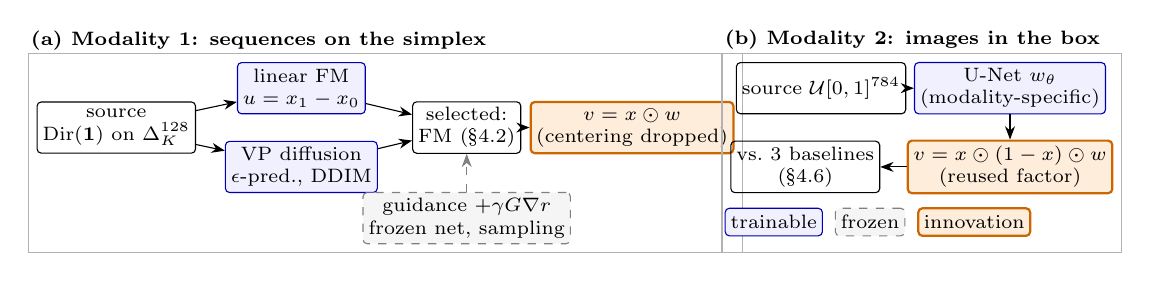
\begin{tikzpicture}[font=\scriptsize, >=Stealth,
  box/.style={draw, rounded corners=1.5pt, align=center, inner sep=2pt, minimum height=6.5mm},
  train/.style={box, draw=blue!70!black, fill=blue!6},
  frozen/.style={box, draw=gray, dashed, fill=gray!8},
  key/.style={box, draw=orange!80!black, fill=orange!14, line width=0.8pt}]
  % (a) Modality 1
  \node[box]    (src) at (0,0)      {source\\$\mathrm{Dir}(\mathbf 1)$ on $\Delta_K^{128}$};
  \node[train]  (fm)  at (2.35,0.5) {linear FM\\$u=x_1-x_0$};
  \node[train]  (df)  at (2.35,-0.5){VP diffusion\\$\epsilon$-pred., DDIM};
  \node[box]    (sel) at (4.45,0)   {selected:\\FM (\S4.2)};
  \node[key]    (inn) at (6.55,0)   {$v=x\odot w$\\(centering dropped)};
  \node[frozen] (gd)  at (4.45,-1.15){guidance $+\gamma G\nabla r$\\frozen net, sampling};
  \draw[->] (src) -- (fm); \draw[->] (src) -- (df);
  \draw[->] (fm) -- (sel); \draw[->] (df) -- (sel); \draw[->] (sel) -- (inn);
  \draw[->, dashed, gray] (gd) -- (sel);
  \node[draw=gray!60, fit=(src)(fm)(df)(sel)(inn)(gd), inner sep=3pt] (pa) {};
  \node[anchor=south west, font=\scriptsize\bfseries, inner sep=1pt] at (pa.north west) {(a) Modality 1: sequences on the simplex};
  % (b) Modality 2
  \node[box]    (s2) at (8.95,0.5)   {source $\mathcal U[0,1]^{784}$};
  \node[train]  (un) at (11.35,0.5)  {U-Net $w_\theta$\\(modality-specific)};
  \node[key]    (i2) at (11.35,-0.5) {$v=x\odot(1-x)\odot w$\\(reused factor)};
  \node[box]    (cp) at (8.75,-0.5)  {vs.\ 3 baselines\\(\S4.6)};
  \draw[->] (s2) -- (un); \draw[->] (un) -- (i2); \draw[->] (i2) -- (cp);
  \node[draw=gray!60, fit=(s2)(un)(i2)(cp)(gd.south -| cp.west), inner sep=3pt] (pb) {};
  \node[anchor=south west, font=\scriptsize\bfseries, inner sep=1pt] at (pb.north west) {(b) Modality 2: images in the box};
  % legend
  \node[train, minimum height=3.5mm]  (l1) at (8.35,-1.2) {trainable};
  \node[frozen, minimum height=3.5mm, right=1.5mm of l1] (l2) {frozen};
  \node[key, minimum height=3.5mm, right=1.5mm of l2] (l3) {innovation};
\end{tikzpicture}

\caption{Study overview. Guidance acts on the frozen network; only the velocity parameterisation
changes, and only the factor is carried to Modality~2. Nothing is pretrained.}
\label{fig:overview}
\end{figure}

\subsection{Modalities, Data, and Preprocessing}
\textbf{Modality 1} is unconditional generation of length-128 sequences, points of
$\Delta_K^{128}$; data are one-hot vertices. \textbf{DNA} ($K=4$): 128-base windows of GRCh38
chr1:1--10\,Mb \citep{ensembl2023}. \textbf{Codon} ($K=64$): the same region in 384-base windows
read as non-overlapping trinucleotides (3-mer tokens, not reading-frame codons). \textbf{Protein}
($K=20$): reviewed human SwissProt entries of length 128--1000 \citep{uniprot2023}, tiled into
non-overlapping 128-residue windows. Held-out sets are split off by protein and by 100\,kb genomic
block (the same blocks for DNA and codon), deduplicated; models train on \MOneTrain{} sequences
and are scored against \MOneHeldout{} held-out ones.
\textbf{Modality 2} is unconditional MNIST \citep{lecun1998mnist} generation in $[0,1]^{784}$,
mapped inside by $x\mapsto0.98x+0.01$; we train on \MTwoTrain{} images and hold out the next
\MTwoEval{} as the Fr\'echet reference. The simplex (a sum-constrained slice) and the box (a
product of intervals) share only boundedness.

\subsection{Continuous Flow Matching Baseline}
With $x_1\sim p_{\text{data}}$ and $x_0\sim\mathrm{Dir}(\mathbf 1)$ per position,
$x_t=(1-t)x_0+tx_1$, $u_t=x_1-x_0$, and
$\mathcal L_{\text{FM}}(\theta)=\mathbb E_{t\sim\mathcal U[0,1]}\lVert v_\theta(x_t,t)-u_t\rVert_2^2$.
The backbone is a dilated 1-D CNN (\MOneLayers{} residual blocks, width \MOneWidth,
\MOneParamsLo--\MOneParamsHi{} parameters); Adam at a constant $10^{-3}$, batch \MOneBatch,
\MOneSteps{} steps, final checkpoint, \MOneSeeds{} seeds. Sampling is Euler at NFE
$\in\{10,50,100\}$, then clamping and renormalisation.

\subsection{Diffusion Baseline}
On the same coordinates, $x_s=\sqrt{\bar\alpha_s}x_1+\sqrt{1-\bar\alpha_s}\,\epsilon$ with the cosine
schedule \citep{nichol2021improved},
$\mathcal L_{\text{diff}}(\phi)=\mathbb E\lVert\epsilon-\epsilon_\phi(x_s,s)\rVert_2^2$, and
deterministic DDIM \citep{song2021ddim},
$x_{s'}=\sqrt{\bar\alpha_{s'}}\hat x_1+\sqrt{1-\bar\alpha_{s'}}\epsilon_\phi$ with
$\hat x_1=(x_s-\sqrt{1-\bar\alpha_s}\epsilon_\phi)/\sqrt{\bar\alpha_s}$. All else matches 3.2.

\subsection{Guided Generation}
We steer the frozen innovation model (\S3.5) toward a sequence property with the reward
$r(x)=\sum_l\log\sum_{i\in S}x_{l,i}$: GC content on DNA ($S=\{\mathrm{C},\mathrm{G}\}$) and
hydrophobic fraction on protein ($S=\{\mathrm{A,I,L,M,F,V,W}\}$). The drift becomes
$x\odot w_\theta+\gamma\nabla r$, $\gamma$ constant in $t$, and each Euler step is projected onto the
simplex and renormalised (the Euclidean rule); nothing is retrained. A synthetic check with an
exact guided law is in App.~\ref{app:guid}.

\subsection{Proposed Innovation}
\emph{Hypothesis:} the learned field points out of the simplex and the repairing clamp distorts
samples, so a field vanishing on each face should generate better. The replicator form
$v=x\odot(w-\langle x,w\rangle)$ \citep{boll2024assignment} combines two mechanisms: $x_i$ makes each
component vanish on the face $x_i=0$, and the centering gives $\sum_iv_i=0$. We propose the factor
alone,
\begin{equation}
v_\theta=x\odot w_\theta(x,t),\qquad
\mathcal L(\theta)=\mathbb E\lVert x_t\odot w_\theta(x_t,t)-(x_1-x_0)\rVert_2^2,
\end{equation}
with no new parameters or hyperparameters; the sum constraint is left to renormalisation. Controls:
the base $v=w$, center-only $v=w-\bar w$ ($\bar w$ the coordinate mean), and the full form (Algorithm~\ref{alg:train}).

\subsection{Transfer to Modality 2}
The invariant idea, a factor vanishing where the domain ends, becomes $v=x\odot(1-x)\odot w$ on the
box (no sum constraint, so no centering). Only the backbone changes: a U-Net (width \MTwoWidth, \MTwoParams{} parameters), uniform source, Adam at
$2\times10^{-4}$, batch 128, \MTwoSteps{} steps, \MTwoSeeds{} seeds, Euler at NFE
$\in\{10,50,100\}$ with violations counted before clamping.

\subsection{Model Overview}
Figure~\ref{fig:overview} summarises what is trained, frozen and changed in each modality.

\section{Results}

\subsection{Evaluation Protocol}
\subsubsection{Metrics}
\emph{Step violation} is the fraction of (sample, step) pairs whose raw Euler update has any of its
$128K$ coordinates below zero, before clamping, with no tolerance. It counts steps, not mass (App.~\ref{app:abl}),
and rises with $K$ through the coordinate count alone, so we compare it within a dataset. Quality is per-position \emph{marginal KL} and \emph{3-mer correlation}
\citep{wang2025drakes}, with a unigram sampler as a floor; diversity is checked post hoc (App.~\ref{app:div}). Modality~2 uses Fr\'echet distance (FD), density and coverage
\citep{naeem2020reliable} in the features of one classifier trained once (\MTwoAcc\% test accuracy).
\subsubsection{Fair Comparison and Computational Budget}
Within an experiment all arms share data, architecture, optimiser, steps, seeds, sample count
(\MOneEval{} sequences; \MTwoEval{} images) and NFE grid; each external method keeps its own path,
objective and decoding (Dirichlet and Gumbel-Softmax train cross-entropy denoisers and decode the
argmax of their final posterior, as published). Seeds fix initialisation, not minibatches across
objectives. Runs used A40 and A6000 GPUs, about \MOneCellMin{} minutes per Modality~1 cell. All
baselines are our re-implementations at our scale; none is quoted.
\subsubsection{Statistical Reporting}
Mean $\pm$ s.d.\ over seeds and paired-bootstrap 95\% intervals (20{,}000 resamples; significant
if the interval excludes zero). At 8 seeds the bootstrap is optimistic, so headline effects also get
Student-$t$ intervals and seed counts; there is no multiplicity correction. Registered before their
runs: Table~\ref{tab:fmdiff_real}, the held-out data and split, the corrected baselines, the
Modality~2 rerun and the guidance test; not registered: the decomposition, the 3-mer endpoint and the choice of datasets.

\subsection{Modality 1: Flow Matching versus Diffusion}
\emph{Which family should carry the innovation?} With the same backbone, flow matching attains
lower held-out marginal KL at every NFE on every dataset, on at least \RealMinWins{} of \RealSeeds{}
seeds (Table~\ref{tab:fmdiff_real}):
\RealCIDna, \RealCIProt{} and \RealCICodon{} (diffusion minus flow matching, NFE 10), and the gap
persists at NFE 100; the preregistered synthetic run agreed (Table~\ref{tab:fmdiff}). Diffusion
was untuned, so we claim the ordering, not the margin; a unigram sampler reaches KL
\UniKLDNA--\UniKLCodon{} on DNA and codon, so this metric mostly tests composition. Diffusion is
also less diverse (Hamming \DiffHam{} vs.\ \FMHam; App.~\ref{app:div}).

\begin{table}[t]
\centering
\caption{Flow matching vs.\ diffusion on the real sequences (\RealSeeds{} seeds): held-out marginal KL and
paired differences, diffusion minus flow matching.}
\label{tab:fmdiff_real}
\footnotesize\begin{adjustbox}{max width=\textwidth}\begin{tabular}{lrrrrr}
\toprule
Dataset & FM, NFE 10 & Diff., NFE 10 & Diff.$-$FM, NFE 10 & Diff.$-$FM, NFE 100 & $x_0$ out (FM / Diff.) \\
\midrule
DNA ($K{=}4$) & 0.0061 $\pm$ 0.0043 & 0.7259 $\pm$ 0.4016 & $\mathbf{+0.720}$ [+0.447, +1.005] & +0.119 [+0.054, +0.194] & 0.979 / 0.993 \\
Protein ($K{=}20$) & 0.3120 $\pm$ 0.0632 & 2.2958 $\pm$ 0.4275 & $\mathbf{+1.984}$ [+1.724, +2.265] & +0.301 [+0.220, +0.391] & 1.000 / 1.000 \\
Codon ($K{=}64$) & 0.7483 $\pm$ 0.1314 & 1.7055 $\pm$ 0.6730 & $\mathbf{+0.957}$ [+0.570, +1.415] & +0.647 [+0.375, +0.991] & 1.000 / 1.000 \\
\bottomrule
\end{tabular}\end{adjustbox}
\end{table}

\begin{table}[t]
\centering
\begin{minipage}[t]{0.49\textwidth}\centering
\caption{Guiding our model (\GRSeeds{} seeds). Hit: above the real 90th percentile;
$r_{\text{top}}$: 3-mer $r$ to the real top decile. Full: Table~\ref{tab:guidance_real_full}.}
\label{tab:guidance_real}
\footnotesize\begin{adjustbox}{max width=\textwidth}\begin{tabular}{lrrrrrr}
\toprule
& \multicolumn{3}{c}{DNA (GC)} & \multicolumn{3}{c}{Protein (hydrophobic)} \\
\cmidrule(lr){2-4}\cmidrule(lr){5-7}
$\gamma$ & Hit$\uparrow$ & $r_{\text{top}}\uparrow$ & Ham. & Hit$\uparrow$ & $r_{\text{top}}\uparrow$ & Ham. \\
\midrule
0 (unguided) & 0.09 & 0.59 & 0.75 & 0.03 & 0.60 & 0.94 \\
0.03 (low) & 0.30 & 0.92 & 0.74 & 0.55 & 0.74 & 0.94 \\
0.3 (default) & 1.00 & 0.65 & 0.53 & 1.00 & 0.53 & 0.84 \\
3 (high) & 1.00 & 0.55 & 0.44 & 1.00 & 0.50 & 0.72 \\
\midrule
\emph{Held-out real} & 0.09 & --- & 0.75 & 0.10 & --- & 0.94 \\
\bottomrule
\end{tabular}\end{adjustbox}
\end{minipage}\hfill
\begin{minipage}[t]{0.49\textwidth}\centering
\caption{Decomposition (\MOneSeeds{} seeds, NFE 100). Bold: significant vs.\ base, or violation
$<10^{-3}$.}
\label{tab:decomp}
\footnotesize\begin{adjustbox}{max width=\textwidth}\begin{tabular}{lrrrrrr}
\toprule
& \multicolumn{3}{c}{3-mer $r$} & \multicolumn{3}{c}{step violation} \\
\cmidrule(lr){2-4}\cmidrule(lr){5-7}
Arm & $K{=}4$ & $K{=}20$ & $K{=}64$ & $K{=}4$ & $K{=}20$ & $K{=}64$ \\
\midrule
base $w$ & 0.894 & 0.753 & 0.127 & 0.713 & 0.967 & 1.000 \\
mult $x \odot w$ & 0.899 & \textbf{0.865} & \textbf{0.196} & \textbf{0.0000} & \textbf{0.0000} & \textbf{0.0000} \\
center $w - \bar{w}$ & 0.910 & 0.777 & 0.120 & 0.721 & 0.967 & 1.000 \\
full replicator & 0.896 & \textbf{0.836} & \textbf{0.187} & 0.010 & 0.010 & 0.016 \\
\bottomrule
\end{tabular}\end{adjustbox}
\end{minipage}
\end{table}

\subsection{Modality 1: Guidance Works}
\emph{Can the frozen model be steered toward a property?} Yes (Table~\ref{tab:guidance_real}). At the
default $\gamma=0.3$ the hit rate rises by \GRHitCIDna{} on DNA and \GRHitCIProt{} on protein
(paired vs.\ unguided), with no violations or extra runtime. The cost is diversity and realism:
Hamming falls by \GRHamCIDna{} and \GRHamCIProt, and samples overshoot real high-property
sequences; post hoc, similarity to the real top decile peaks at small strength ($\gamma=\GRBestGammaDna$
on DNA: \GRKmerHiMidDna{} vs.\ \GRKmerHiZeroDna{} unguided).


\subsection{Modality 1: Innovation Ablations}
\emph{Which part of the replicator form matters?} The base field leaves the simplex on
\BaseViolDna, \BaseViolProt{} and \BaseViolCodon{} of steps at $K=4,20,64$ (NFE 100;
Fig.~\ref{fig:kscaling}; per coordinate it falls). In
Table~\ref{tab:decomp} (Fig.~\ref{fig:decomp}) the factor alone improves 3-mer correlation by \MultCIProt{} at $K=20$
and \MultCICodon{} at $K=64$ (\MultProtPos/\MultProtN{} and \MultCodonPos/\MultCodonN{} seeds; $t$-intervals agree); center-only
is never significant (the base target already sums to zero), and dropping the full form's centering
changes nothing (\DropCenterCICodon). Violations vanish at NFE $\ge50$; at NFE 10
\MultViolTenLo--\MultViolTenHi\% remain, about one step in ten. At $K=20$ the gain shrinks with NFE (\MultMeanProtTen, \MultMeanProtFifty,
\MultMeanProtHundred), as a clamping effect would; at $K=64$ it is not significant at NFE 10
(\MultCICodonTen) and appears from NFE 50 (Fig.~\ref{fig:nfe}).


\subsection{Modality 1: Comparison with Recent Methods}
\emph{Is the method competitive?} No (Table~\ref{tab:baselines}, Fig.~\ref{fig:baselines}). At
$K=4$ all are within noise; at $K=20,64$ Dirichlet flow matching leads us by \DirichletVsOursProt{}
and \DirichletVsOursCodon, Fisher-Flow by \FisherVsOursProt{} and \FisherVsOursCodon; we beat
Gumbel-Softmax only at $K=20$. All three are feasible in their own samplers (App.~\ref{app:base}). A
no-model unigram sampler scores \UniProtein{} and \UniCodon{} at $K=20,64$: protein 3-mer correlation
is nearly saturated by composition, and on codon ours (\OursKmerCodon) stays below the floor.

\begin{table}[t]
\centering
\caption{Recent methods (our re-implementations), the base and a no-model reference
(\MOneSeeds{} seeds, NFE 100). Violation is of each method's own update.}
\label{tab:baselines}
\footnotesize\begin{adjustbox}{max width=\textwidth}\begin{tabular}{lrrrr}
\toprule
& \multicolumn{3}{c}{3-mer $r$ $\uparrow$ (NFE 100)} & Step viol. $\downarrow$ \\
\cmidrule(lr){2-4}
Method & DNA ($K{=}4$) & Protein ($K{=}20$) & Codon ($K{=}64$) & $K{=}4/20/64$ \\
\midrule
Dirichlet FM~\citep{stark2024dirichlet} & 0.901 $\pm$ 0.062 & 0.906 $\pm$ 0.020 & 0.447 $\pm$ 0.020 & 0.00/0.00/0.00 \\
Fisher-Flow~\citep{davis2024fisher} & 0.909 $\pm$ 0.049 & 0.886 $\pm$ 0.016 & 0.295 $\pm$ 0.013 & 0.00/0.00/0.00 \\
Gumbel-Softmax FM~\citep{tang2025gumbel} & 0.894 $\pm$ 0.052 & 0.705 $\pm$ 0.061 & 0.400 $\pm$ 0.070 & 0.00/0.00/0.00 \\
\midrule
Linear FM (internal base) & 0.894 $\pm$ 0.088 & 0.753 $\pm$ 0.058 & 0.127 $\pm$ 0.023 & 0.71/0.97/1.00 \\
\textbf{Ours}: $v = x \odot w$ & 0.899 $\pm$ 0.061 & 0.865 $\pm$ 0.027 & 0.196 $\pm$ 0.016 & 0.00/0.00/0.00 \\
\midrule
\emph{Reference: unigram sampler (no model)} & -0.046 $\pm$ 0.025 & 0.900 $\pm$ 0.002 & 0.218 $\pm$ 0.002 & --- \\
\bottomrule
\end{tabular}\end{adjustbox}
\end{table}

\subsection{Modality 2: Transfer of the Innovation}
\emph{Does the factor help in a different state space?} Feasibility transfers (violation
\MTwoViolOurs; Table~\ref{tab:m2}, Fig.~\ref{fig:m2fig}); quality does not. The paired FD change
against the base is \MTwoClaim, so the preregistered claim fails; ours matches reflection and
thresholding, which act as plain clamping \citep{lou2023reflected}, is significantly worse than
mirror-map flow matching (\MTwoVsMirror), and loses coverage and density on all \MTwoSeeds{} seeds.
Mirror also uses a different source (Gaussian in logit space).

\begin{table}[t]
\centering
\caption{Transfer to MNIST (\MTwoSeeds{} seeds, NFE 100 unless noted). All arms are flow matching
in our harness: reflection and thresholding are sampler rules; mirror trains in logit space.}
\label{tab:m2}
\footnotesize\begin{adjustbox}{max width=\textwidth}\begin{tabular}{lrrrrr}
\toprule
Method & FD $\downarrow$ & Coverage $\uparrow$ & Density $\uparrow$ & FD@10 $\downarrow$ & Step viol. $\downarrow$ \\
\midrule
Reflection sampler~\citep{lou2023reflected} & 192.0 $\pm$ 143.5 & 0.624 & 0.478 & 540.3 & 0.1401 \\
Mirror-map FM~\citep{liu2023mirror} & 52.5 $\pm$ 23.9 & 0.685 & 0.480 & 98.9 & 0.0000 \\
Dyn.\ thresholding on $x_t$~\citep{saharia2022imagen} & 195.5 $\pm$ 150.3 & 0.623 & 0.480 & 540.8 & 0.1604 \\
\midrule
Flow matching (internal base) & 193.9 $\pm$ 145.6 & 0.623 & 0.478 & 545.3 & 0.1602 \\
\textbf{Ours}: $v = x(1-x)\odot w$ & 151.0 $\pm$ 47.4 & 0.410 & 0.302 & 269.6 & 0.0000 \\
\bottomrule
\end{tabular}\end{adjustbox}
\end{table}

\subsection{Cross-Modality Analysis and Failure Modes}
\emph{Does the mechanism help for the same reason in both spaces?} The factor removes violations in
both, but feasibility does not separate methods: every strong one is feasible (by vanishing
mixtures, a change of coordinates or our factor) yet quality differs widely. Failure modes: protein
barely exceeds composition; on images coverage and density fall and samples are blotchier
(Fig.~\ref{fig:m2samples}); at NFE 10 the last step overshoots; six interventions failed
(Table~\ref{tab:interventions}). \emph{Answer:} the factor improves the linear base at $K\ge20$,
trails recent methods, and transfers feasibility but not quality.

\section{Discussion}
The ablation shows causally that the factor, not the centering, is the active part; the baseline
and transfer comparisons are correlational and go against us. The likeliest explanation of the gain
is an inductive bias: multiplying by $x_i$ concentrates the field where mass already is, as the
Dirichlet and Gumbel mixtures also do; its decay with NFE at $K=20$ suggests part is avoided clamping.

Limitations: small models, re-implemented baselines, post-hoc diversity checks and a protein metric
near its composition floor. Supported: a vanishing factor removes violation at NFE $\ge50$ and
improves a linear flow at $K\ge20$; its centering is unnecessary; it trails recent methods.

\bibliographystyle{ieeetr}
\bibliography{refs}

\newpage
\appendix
\renewcommand{\thetable}{S\arabic{table}}\setcounter{table}{0}
\renewcommand{\thefigure}{S\arabic{figure}}\setcounter{figure}{0}
\section{Appendix}
Every table and figure here supports the main text: Table~\ref{tab:fmdiff} (\S4.2),
Table~\ref{tab:guidance_full} (\S4.3), Figures~\ref{fig:kscaling}, \ref{fig:nfe} and~\ref{fig:decomp}
(\S4.4), Figure~\ref{fig:baselines} (\S4.5), Figures~\ref{fig:m2fig} and~\ref{fig:m2samples}
(\S4.6--4.7) and Table~\ref{tab:interventions} (\S4.7).

\subsection{Dataset and Preprocessing Details}
Built by \texttt{experiments/prepare\_real\_data\_v2.py}; array hashes are in
\texttt{results/data\_v2\_manifest.json}. DNA and codon come from one region, GRCh38
chr1:1{,}000{,}000--9{,}999{,}999 (Ensembl REST, upper-cased), cut into 128- and 384-base windows;
windows containing \texttt{N} are dropped. 18 of 90 blocks of 100\,kb are held out, the same for
both, and windows straddling a train/held-out boundary are dropped. Protein uses the 16{,}363
reviewed human SwissProt entries of length 128--1000, tiled from the N-terminus into
non-overlapping 128-residue windows (windows with non-standard residues dropped); 20\% of
accessions are held out, so no protein contributes to both sides. Exact duplicates are removed
within each side and held-out windows identical to a training window are removed. Pools are
38{,}300/9{,}746 (protein), 56{,}236/13{,}709 (DNA) and 18{,}733/4{,}559 (codon) train/held-out
windows, each permuted (seed 0) and truncated to \MOneTrain/\MOneHeldout. An earlier version kept only
each protein's first 128 residues and split nothing; it is superseded. MNIST uses the standard
60{,}000 training images.

\subsection{Training and Sampling Details}
Modality~1 CNN: kernel 5, dilation cycling $1,2,4,8,16$, GroupNorm, sinusoidal time features,
zero-initialised output. Modality~2 U-Net: two downsampling stages (width \MTwoWidth{} and twice
that), a mid block and symmetric upsampling with skip connections, GroupNorm, SiLU, sinusoidal
time embedding per block. The mirror baseline trains flow matching on $y=\mathrm{logit}(x)/4$
from a Gaussian source and maps back through the sigmoid, so its source differs from the other
arms'. No run uses a learning-rate schedule, early stopping or checkpoint selection.

\subsection{Additional Ablations}
\label{app:abl}
Table~\ref{tab:fmdiff} is the preregistered \S4.2 decision run. It deviated from our registration,
which specified the dilated CNN and a real-data leg; the deviation is disclosed in the repository's
preregistration log, and Table~\ref{tab:fmdiff_real} is the registered repair.
Table~\ref{tab:interventions} lists the other constraint interventions we tried; with the
Modality~2 transfer, six interventions were falsified, including a soft tangency penalty, a
convex-combination integrator (a no-op under uniform steps) and a $(1-t)^2$ loss reweighting that
was harmful against the base (\ReweightCIProt{} at $K=20$; the $t$-interval \ReweightProtT{}
includes zero, \ReweightProtPos/\ReweightProtN{} seeds favour it).
\textbf{Violation magnitude and step size.} On a synthetic $K=\SweepK$ model the base rate is flat
(\SweepRateLo--\SweepRateHi) over a $\SweepRatio\times$ step-size range and the clamped mass is
$\SweepMassLo$--$\SweepMassHi$ per step; on real DNA the rate rises from \BaseViolDnaTen{} at NFE 10.
We did not measure clamped mass on real data.

\begin{table}[h]
\centering
\caption{The preregistered \S4.2 decision run: synthetic categorical target, small MLP,
\SynSeeds{} seeds. Marginal KL (lower better).}
\label{tab:fmdiff}
\resizebox{\textwidth}{!}{\begin{tabular}{lrrrrrr}
\toprule
Method & $K{=}4$, NFE 10 & $K{=}4$, NFE 100 & $K{=}60$, NFE 10 & $K{=}60$, NFE 100 & $x_0$ out, $K{=}4$ & $x_0$ out, $K{=}60$ \\
\midrule
Flow matching & 0.0232 $\pm$ 0.0096 & 0.0101 $\pm$ 0.0040 & 0.1873 $\pm$ 0.0406 & 0.0635 $\pm$ 0.0103 & 0.795 & 1.000 \\
Diffusion (VP, DDIM) & 0.2436 $\pm$ 0.1312 & 0.0414 $\pm$ 0.0424 & 0.2708 $\pm$ 0.0741 & 0.1636 $\pm$ 0.0949 & 0.789 & 1.000 \\
\bottomrule
\end{tabular}}
\end{table}

\begin{table}[h]
\centering
\caption{Constraint interventions (NFE 100): what each fixes and what it costs.}
\label{tab:interventions}
\small
\begin{tabular}{llrrr}
\toprule
Alphabet & Arm & Step viol. & $x_0$ outside & 3-mer $r$ \\
\midrule
DNA & unconstrained & 0.7132 & 0.9785 & 0.8943 $\pm$ 0.0876 \\
DNA & hard & 0.0098 & 0.9219 & 0.8961 $\pm$ 0.0409 \\
DNA & endpoint & 0.0000 & 0.0022 & 0.8543 $\pm$ 0.0405 \\
\midrule
Protein & unconstrained & 0.9667 & 1.0000 & 0.7526 $\pm$ 0.0576 \\
Protein & hard & 0.0103 & 0.9980 & 0.8360 $\pm$ 0.0370 \\
Protein & endpoint & 0.0100 & 0.6385 & 0.5019 $\pm$ 0.3607 \\
\midrule
Codon & unconstrained & 1.0000 & 1.0000 & 0.1268 $\pm$ 0.0233 \\
Codon & hard & 0.0159 & 1.0000 & 0.1874 $\pm$ 0.0396 \\
Codon & endpoint & 0.0100 & 0.7245 & 0.0714 $\pm$ 0.0816 \\
\bottomrule
\end{tabular}
\end{table}

\begin{figure}[h]
\centering
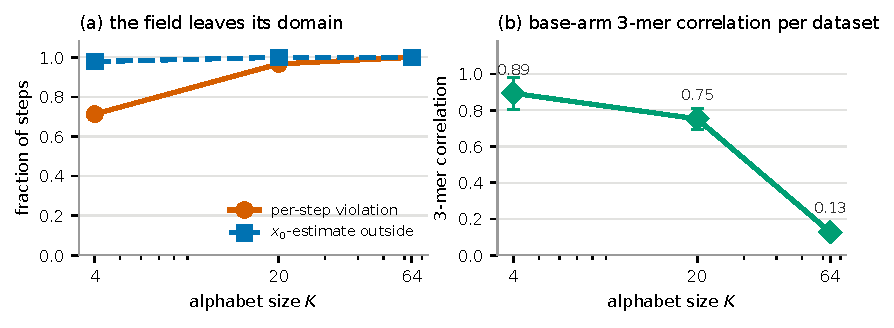
\includegraphics[width=0.9\textwidth]{figures/fig2_kscaling.pdf}
\caption{Non-tangency of the base arm against alphabet size (Table~\ref{tab:decomp}, base rows).}
\label{fig:kscaling}
\end{figure}

\begin{figure}[h]
\centering
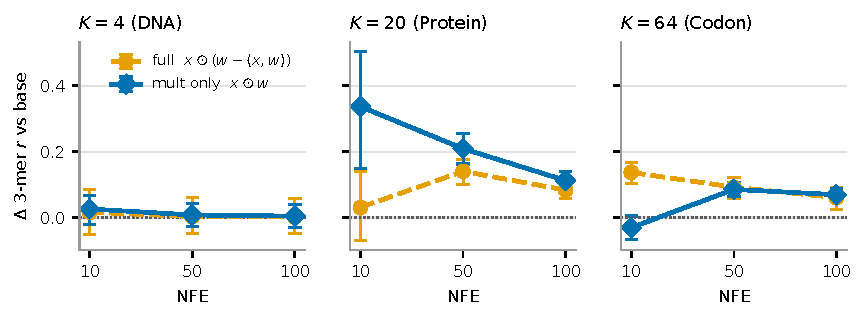
\includegraphics[width=0.9\textwidth]{figures/fig3_nfe.pdf}
\caption{Gain over the base against NFE. Dashed: full replicator. Solid: multiplicative factor
alone. At $K{=}20$ both gains shrink as steps shrink; at $K{=}64$ the factor's gain appears only
from NFE 50.}
\label{fig:nfe}
\end{figure}

\begin{figure}[h]
\centering
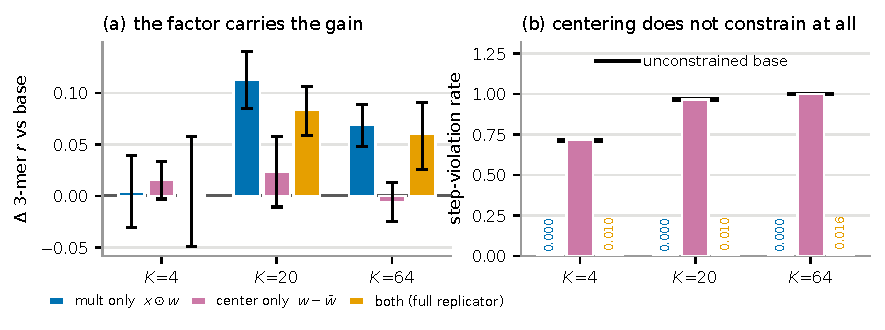
\includegraphics[width=0.9\textwidth]{figures/fig4_decomposition.pdf}
\caption{One-at-a-time removal of the two pieces of the replicator form (Table~\ref{tab:decomp}).}
\label{fig:decomp}
\end{figure}

\subsection{Additional Baseline Results}
\label{app:base}
All baseline numbers are reproduced by our group; none is quoted from the original papers.
\textbf{Corrections, each preregistered before its run.} (i) Our first Fisher-Flow sampler integrated
its sphere velocity in simplex coordinates; the corrected arm steps on the sphere and maps back by
$p=s^2$, so its own update is feasible by construction (as a Euclidean simplex velocity its field
would exit on \FisherViolEuclid{} of steps; exponential-map steps can still leave the positive
orthant of the sphere). (ii) Our first Dirichlet and Gumbel-Softmax arms regressed on velocity
targets that were neither the published methods nor their own paths' velocities (Gumbel's was
$18.4\times$ too small). They now train the published cross-entropy denoisers with the published
conditional fields (the Dirichlet $C$-factor as in the authors' code) and decode, as published, the
argmax of the final posterior. Neither path reaches a vertex, so decoding the final state instead
gives lower scores at large $K$: 3-mer $r$ \GumbelKmerState{} (Gumbel) and \DirichletKmerState{}
(Dirichlet). (iii) All Modality~1 numbers were first scored against the training sequences, on
data that kept only protein N-termini; they are now scored on held-out rebuilt data. The
train-minus-held-out 3-mer gap is small (\TrainGapBase{} base, \TrainGapOurs{} ours). (iv)
Modality~2 first used one feature extractor per run; one shared extractor now scores every arm, and
no verdict changed. (v) A guidance rule described as an entropic mirror step was the
natural-gradient update, and a stale natural-gradient violation rate was replaced by a rerun.
Superseded rows remain in the repository (e.g.\ training-reference 3-mer $r$ of the first
implementations: Dirichlet \DirichletKmerOld, Gumbel \GumbelKmerOld, Fisher \FisherKmerOld).


\begin{figure}[h]
\centering
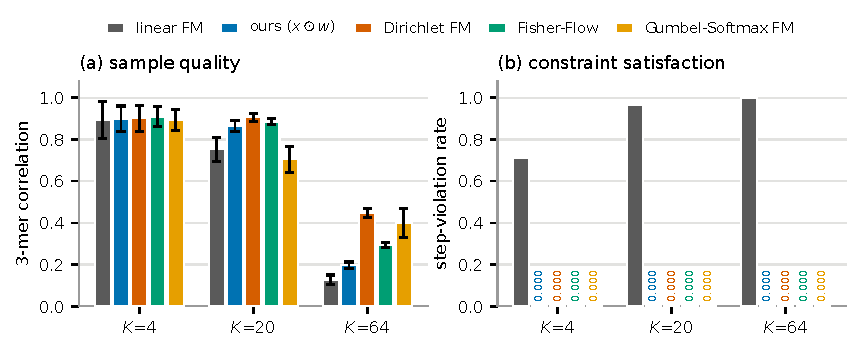
\includegraphics[width=0.9\textwidth]{figures/fig5_baselines.pdf}
\caption{Matched comparison with recent methods (Table~\ref{tab:baselines} in graphical form).}
\label{fig:baselines}
\end{figure}

\begin{figure}[h]
\centering
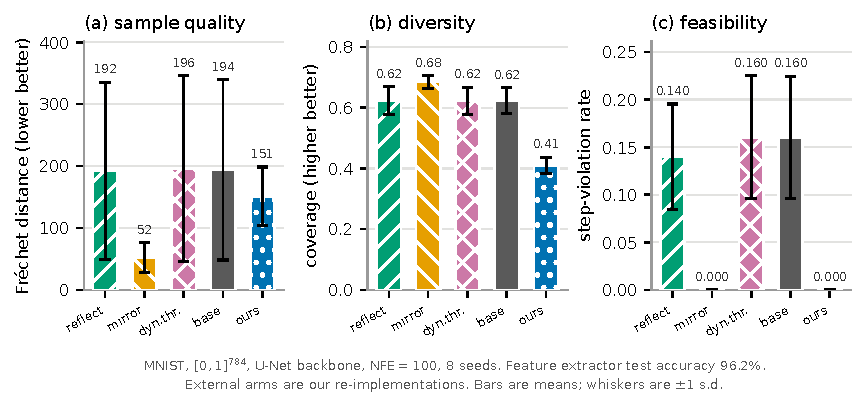
\includegraphics[width=0.9\textwidth]{figures/fig6_modality2.pdf}
\caption{Modality~2 transfer (Table~\ref{tab:m2} in graphical form).}
\label{fig:m2fig}
\end{figure}

\subsection{Guidance: Full Grid and Synthetic Check}
\label{app:guid}
Table~\ref{tab:guidance_real_full} gives every guidance strength on the real sequences. The
synthetic check guides a base model on one position with $K=\GuidK$ toward the two rarest
symbols, where the ideal guided law ($p_{\text{data}}$ restricted to $S$) is known exactly. Unguided,
$S$ is hit with probability \GuidHitZero; every rule reaches \GuidHitMax{} by $\gamma=8$ with KL to the
ideal law of \GuidKLLo--\GuidKLHi{} (Table~\ref{tab:guidance}; \GuidN{} samples). At $\gamma=8$ the
tangent rule escapes with $\GuidMassRatio\times$ the Euclidean rule's mass, and the natural gradient
cuts the violation rate from \GuidViolEuc{} to \GuidViolNat{} but needs $\GuidStrengthRatio\times$ the
strength. At $\gamma=0$ the rate is already \GuidViolZero: the base field, not guidance, leaves the
domain.

\begin{table}[h]
\centering
\caption{Real-data guidance, full $\gamma$ grid (\GRSeeds{} seeds).}
\label{tab:guidance_real_full}
\footnotesize\begin{adjustbox}{max width=\textwidth}\begin{tabular}{llrrrrr}
\toprule
Property & Guidance ($\gamma$) & Target frac.\ $\uparrow$ & Hit rate $\uparrow$ & 3-mer $r$ held-out & 3-mer $r$ top decile $\uparrow$ & Hamming (diversity) \\
\midrule
DNA (GC) & 0 & 0.510 $\pm$ 0.026 & 0.09 $\pm$ 0.05 & 0.901 $\pm$ 0.058 & 0.588 $\pm$ 0.156 & 0.748 $\pm$ 0.002 \\
 & 0.01 & 0.537 $\pm$ 0.025 & 0.14 $\pm$ 0.07 & 0.859 $\pm$ 0.073 & 0.749 $\pm$ 0.104 & 0.746 $\pm$ 0.003 \\
 & 0.03 & 0.589 $\pm$ 0.023 & 0.30 $\pm$ 0.10 & 0.715 $\pm$ 0.071 & 0.916 $\pm$ 0.041 & 0.740 $\pm$ 0.005 \\
 & 0.1 & 0.742 $\pm$ 0.018 & 0.93 $\pm$ 0.03 & 0.368 $\pm$ 0.033 & 0.939 $\pm$ 0.029 & 0.689 $\pm$ 0.009 \\
 & 0.3 & 0.961 $\pm$ 0.005 & 1.00 $\pm$ 0.00 & 0.040 $\pm$ 0.011 & 0.649 $\pm$ 0.020 & 0.533 $\pm$ 0.008 \\
 & 1 & 1.000 $\pm$ 0.000 & 1.00 $\pm$ 0.00 & 0.038 $\pm$ 0.023 & 0.579 $\pm$ 0.058 & 0.469 $\pm$ 0.051 \\
 & 3 & 1.000 $\pm$ 0.000 & 1.00 $\pm$ 0.00 & 0.043 $\pm$ 0.028 & 0.553 $\pm$ 0.068 & 0.438 $\pm$ 0.069 \\
 & \emph{held-out real} & 0.495 & 0.09 & --- & --- & --- \\
\midrule
Protein (hydrophobic) & 0 & 0.356 $\pm$ 0.011 & 0.03 $\pm$ 0.01 & 0.855 $\pm$ 0.039 & 0.598 $\pm$ 0.054 & 0.943 $\pm$ 0.001 \\
 & 0.01 & 0.390 $\pm$ 0.014 & 0.12 $\pm$ 0.05 & 0.823 $\pm$ 0.062 & 0.675 $\pm$ 0.058 & 0.943 $\pm$ 0.001 \\
 & 0.03 & 0.455 $\pm$ 0.017 & 0.55 $\pm$ 0.13 & 0.697 $\pm$ 0.084 & 0.742 $\pm$ 0.067 & 0.941 $\pm$ 0.001 \\
 & 0.1 & 0.639 $\pm$ 0.021 & 1.00 $\pm$ 0.00 & 0.383 $\pm$ 0.061 & 0.683 $\pm$ 0.058 & 0.921 $\pm$ 0.004 \\
 & 0.3 & 0.951 $\pm$ 0.015 & 1.00 $\pm$ 0.00 & 0.217 $\pm$ 0.020 & 0.532 $\pm$ 0.022 & 0.841 $\pm$ 0.011 \\
 & 1 & 1.000 $\pm$ 0.000 & 1.00 $\pm$ 0.00 & 0.275 $\pm$ 0.015 & 0.531 $\pm$ 0.035 & 0.747 $\pm$ 0.037 \\
 & 3 & 1.000 $\pm$ 0.000 & 1.00 $\pm$ 0.00 & 0.269 $\pm$ 0.022 & 0.495 $\pm$ 0.054 & 0.715 $\pm$ 0.057 \\
 & \emph{held-out real} & 0.351 & 0.10 & --- & --- & --- \\
\bottomrule
\end{tabular}\end{adjustbox}
\end{table}

\begin{table}[h]
\centering
\caption{Synthetic guidance check, $K{=}\GuidK$ target (one seed). Full sweep:
Table~\ref{tab:guidance_full}.}
\label{tab:guidance}
\footnotesize\begin{tabular}{lrrrrrr}
\toprule
& \multicolumn{3}{c}{$\gamma = 1$} & \multicolumn{3}{c}{$\gamma = 8$} \\
\cmidrule(lr){2-4}\cmidrule(lr){5-7}
Rule & Hit $\uparrow$ & KL $\downarrow$ & Viol. $\downarrow$ & Hit $\uparrow$ & KL $\downarrow$ & Viol. $\downarrow$ \\
\midrule
Unguided ($\gamma{=}0$) & 0.0136 & 4.30 & 0.210 & --- & --- & --- \\
\midrule
euclidean & 0.9994 & 0.071 & 0.884 & 1.0000 & 0.048 & 0.972 \\
tangent & 0.9995 & 0.070 & 0.977 & 1.0000 & 0.046 & 1.000 \\
natural & 0.4811 & 0.735 & 0.267 & 1.0000 & 0.066 & 0.766 \\
\bottomrule
\end{tabular}
\end{table}

\subsection{Additional Samples and Failure Cases}
\label{app:div}
\textbf{Diversity (exploratory, added after the results).} Marginal KL and 3-mer correlation cannot
see a generator that repeats a few sequences, so from the saved NFE-100 samples (4{,}000 per cell)
we measure the unique-sequence fraction and the mean pairwise normalised Hamming distance
(Table~\ref{tab:diversity}); Hamming distance tracks composition, so the target is the held-out
value, not the largest. Base, ours, the ablations, Dirichlet FM and Fisher-Flow match held-out
data. The endpoint arms \emph{collapse}: on \EndpointCollapseProt{} of 8 protein and
\EndpointCollapseCodon{} of 8 codon seeds (reweighted: \EndpointRwCollapseProt{} and
\EndpointRwCollapseCodon) every sample is the same sequence, which is what their low, erratic
3-mer scores reflect. Gumbel-Softmax FM decoded by its posterior is less diverse than the data
(Hamming \GumbelHamProt{} vs \RealHamProt{} on protein, \GumbelHamCodon{} vs \RealHamCodon{} on
codon); decoded by its state it matches (\GumbelStateHamProt). No arm reproduces a training sequence
(largest exact-copy rate \MaxTrainCopy). For guidance, where the state is one symbol, the analogue is
the split between the two target symbols: the ideal law puts \GuidRareIdeal\% of the target mass
on the rarer one; at $\gamma=8$ the Euclidean and tangent rules put \GuidRareEuc\% and
\GuidRareTan\% (under-dispersed), the natural gradient \GuidRareNat\% (over-dispersed). None collapses
onto one symbol.

\begin{table}[h]
\centering
\caption{Exploratory diversity, Modality~1 (8 seeds, 4{,}000 samples, NFE 100; mean $\pm$ s.d.).
Denoiser baselines decoded by their posterior, as reported elsewhere. $^\dagger$A sample-saving rerun
of the \S4.2 families; it reproduces the registered marginal KL exactly.}
\label{tab:diversity}
\footnotesize\begin{adjustbox}{max width=\textwidth}\begin{tabular}{lrrrrrr}
\toprule
& \multicolumn{3}{c}{Pairwise Hamming (NFE 100)} & \multicolumn{3}{c}{Unique fraction} \\
\cmidrule(lr){2-4}\cmidrule(lr){5-7}
Arm & DNA & Protein & Codon & DNA & Protein & Codon \\
\midrule
\emph{Held-out real} & 0.750 $\pm$ 0.000 & 0.940 $\pm$ 0.000 & 0.982 $\pm$ 0.000 & 1.00 & 1.00 & 1.00 \\
\emph{Unigram (no model)} & 0.750 $\pm$ 0.000 & 0.941 $\pm$ 0.000 & 0.982 $\pm$ 0.000 & 1.00 & 1.00 & 1.00 \\
\midrule
Linear FM (base) & 0.747 $\pm$ 0.003 & 0.944 $\pm$ 0.001 & 0.980 $\pm$ 0.002 & 1.00 & 1.00 & 1.00 \\
Ours $x\odot w$ & 0.748 $\pm$ 0.002 & 0.944 $\pm$ 0.001 & 0.982 $\pm$ 0.001 & 1.00 & 1.00 & 1.00 \\
Center-only & 0.748 $\pm$ 0.003 & 0.943 $\pm$ 0.001 & 0.980 $\pm$ 0.003 & 1.00 & 1.00 & 1.00 \\
Full replicator & 0.748 $\pm$ 0.001 & 0.944 $\pm$ 0.001 & 0.982 $\pm$ 0.001 & 1.00 & 1.00 & 1.00 \\
Endpoint & 0.749 $\pm$ 0.000 & 0.588 $\pm$ 0.455 & 0.368 $\pm$ 0.475 & 1.00 & 0.63 & 0.38 \\
Endpoint, reweighted & 0.749 $\pm$ 0.001 & 0.587 $\pm$ 0.454 & 0.245 $\pm$ 0.424 & 1.00 & 0.63 & 0.25 \\
Dirichlet FM & 0.748 $\pm$ 0.002 & 0.939 $\pm$ 0.002 & 0.981 $\pm$ 0.001 & 1.00 & 1.00 & 1.00 \\
Fisher-Flow & 0.748 $\pm$ 0.001 & 0.941 $\pm$ 0.002 & 0.981 $\pm$ 0.001 & 1.00 & 1.00 & 1.00 \\
Gumbel-Softmax FM & 0.746 $\pm$ 0.003 & 0.878 $\pm$ 0.011 & 0.947 $\pm$ 0.004 & 1.00 & 1.00 & 1.00 \\
\midrule
Flow matching, NFE 10$^\dagger$ & 0.747 $\pm$ 0.002 & 0.911 $\pm$ 0.023 & 0.872 $\pm$ 0.081 & 1.00 & 1.00 & 1.00 \\
Diffusion (DDIM)$^\dagger$ & 0.687 $\pm$ 0.042 & 0.896 $\pm$ 0.049 & 0.941 $\pm$ 0.034 & 1.00 & 1.00 & 1.00 \\
Diffusion, NFE 10$^\dagger$ & 0.464 $\pm$ 0.157 & 0.602 $\pm$ 0.136 & 0.786 $\pm$ 0.217 & 1.00 & 1.00 & 1.00 \\
\bottomrule
\end{tabular}\end{adjustbox}
\end{table}

\begin{figure}[h]
\centering
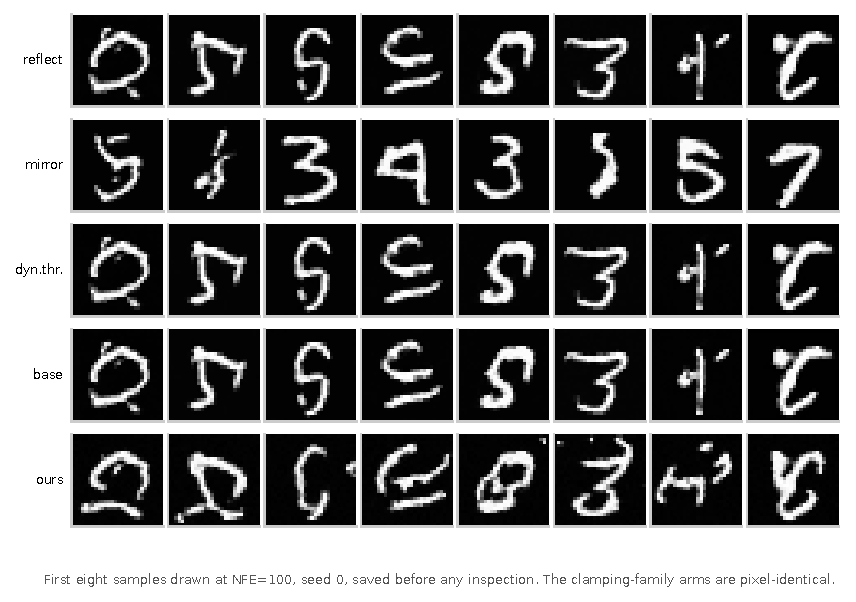
\includegraphics[width=0.8\textwidth]{figures/fig7_m2_samples.pdf}
\caption{Uncurated Modality~2 samples (the first eight drawn at NFE 100, seed \MTwoSampleSeed, saved before
inspection). Our arm attains a lower FD than the base on this seed yet is visibly blotchier: FD in
a small classifier's features is not a perceptual judgement.}
\label{fig:m2samples}
\end{figure}

\begin{table}[h]
\centering
\caption{Full guidance sweep; Table~\ref{tab:guidance} reports the $\gamma\in\{1,8\}$ columns.}
\label{tab:guidance_full}
\small
\begin{tabular}{lrrrr}
\toprule
Rule & $\gamma$ & Hit rate $\uparrow$ & KL to ideal $\downarrow$ & Step viol. $\downarrow$ \\
\midrule
euclidean & 0.0 & 0.0136 & 4.2978 & 0.2102 \\
euclidean & 0.5 & 0.5642 & 0.6748 & 0.7134 \\
euclidean & 1.0 & 0.9994 & 0.0710 & 0.8837 \\
euclidean & 2.0 & 1.0000 & 0.0646 & 0.9293 \\
euclidean & 4.0 & 1.0000 & 0.0513 & 0.9541 \\
euclidean & 8.0 & 1.0000 & 0.0478 & 0.9723 \\
\midrule
tangent & 0.0 & 0.0140 & 4.2695 & 0.2106 \\
tangent & 0.5 & 0.5674 & 0.6728 & 0.9479 \\
tangent & 1.0 & 0.9995 & 0.0698 & 0.9772 \\
tangent & 2.0 & 1.0000 & 0.0655 & 0.9921 \\
tangent & 4.0 & 1.0000 & 0.0514 & 0.9982 \\
tangent & 8.0 & 1.0000 & 0.0461 & 0.9999 \\
\midrule
natural & 0.0 & 0.0138 & 4.2810 & 0.2104 \\
natural & 0.5 & 0.1264 & 2.0826 & 0.1691 \\
natural & 1.0 & 0.4811 & 0.7355 & 0.2674 \\
natural & 2.0 & 0.9430 & 0.1072 & 0.4950 \\
natural & 4.0 & 1.0000 & 0.0588 & 0.6660 \\
natural & 8.0 & 1.0000 & 0.0665 & 0.7662 \\
\bottomrule
\end{tabular}
\end{table}

\textbf{Commitment time.} The decoded $\arg\max$ of $x_t$ settles early: mean settling times are
\CommitDna, \CommitProt{} and \CommitCodon{} for $K=4,20,64$, with
\CommitSettledLo--\CommitSettledHi\% of positions settled by $t=0.25$. This is a different
quantity from the posterior in St\"ark et al.~\citep[Prop.~1]{stark2024dirichlet}, which is an upper bound, and
under a $\mathrm{Dir}(\mathbf 1)$ source much of it follows from the geometry of the linear path
rather than from the model. We report it as descriptive only.

\subsection{Algorithms}
\label{app:alg}
\begin{algorithm}[h]
\caption{Training and sampling with the multiplicative factor ($\theta$ is the only trainable component)}
\label{alg:train}
\begin{algorithmic}[1]
\For{$k=1,\dots,$ \MOneSteps}
  \State sample $x_1\sim\mathcal D$ (one-hot), $x_0\sim\mathrm{Dir}(\mathbf 1)$ per position, $t\sim\mathcal U[0,1]$
  \State $x_t\gets(1-t)x_0+tx_1$;\quad $v\gets x_t\odot w_\theta(x_t,t)$ \Comment{box: $x_t\odot(1-x_t)\odot w_\theta$}
  \State $\theta\gets\theta-\eta\nabla_\theta\lVert v-(x_1-x_0)\rVert_2^2$
\EndFor
\State \textbf{Sample:} $x\sim\mathrm{Dir}(\mathbf 1)$; for $i=0,\dots,N-1$: $x\gets x+\tfrac1N\,x\odot w_\theta(x,\tfrac iN)$, clamp at $0$, renormalise
\State \Return $\arg\max$ per position
\end{algorithmic}
\end{algorithm}

\subsection{Implementation and Reproducibility Details}
Every table, figure and in-text number is regenerated from the stored result files by
\texttt{scripts/make\_tables.py} and \texttt{scripts/make\_figures.py}; the repository README maps
each script to the tables it produces and gives setup, data preparation and run commands.
PyTorch~2.8 with CUDA 12.8 on the rented GPUs and MPS locally; seeds $0$--$7$; the Gamma sampler
used by the Dirichlet baseline was validated against \texttt{scipy} by Kolmogorov--Smirnov test
($p=\GammaKSp$ at shapes \GammaShapes). Baselines are re-implemented from their papers; the
Dirichlet $C$-factor follows the authors' reference code and matches it to $10^{-10}$.

\end{document}
